%!TEX root = main.tex
\section{Introduction }
Machine learning is an emerging field that deals with the development of algorithms which can predict and classify novelties based on a set of prior “intuitions” \cite{mlsurvey}. The field incorporates ideas from biology, computer science, numerical analysis, and statistics. In recent years machine learning has entered the main stream through web services like Google, Facebook, and Amazon. There is an incentive from both academia and industry to expand machine learning techniques and applications. 

One of the most popular algorithms of the field is the artificial neural network (ANN). Although there are numerous mathematical interpretations of neural networks, we will primarily focus on the expansion of one type, feed-forward neural networks. As ANNs are based off the structure of biological neurons, a biological approach is necessary to understand this interpretation.
\subsection{Biological Neuron}
A single neuron consists of the cell body (the soma), the dendrites, and the axon. Mathematically we wish to examine the process of neural activation, the events which lead to the excitation of the axon. Consider a neuron that has activated anterior neurons (those which are connected dendritically); that is, the neuron is receiving input along all of its dendrites. These electrical inputs propagate through the dendrites and become integrated on the soma as electrical membrane potential \cite{griffith}. The soma then acts as the primary computational unit and activates the axon when a threshold of input activity is reached. More specifically, when a membrane potential of about -60 mV is reached on the soma, the hillock zone, or axon hillock, activates the axon by applying proteins to an ion channel which creates action potential along the axon \cite{bioneuron}.
\subsection{Artificial Neurons}
\begin{figure}
\centering
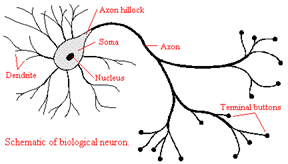
\includegraphics{neuron}
\caption{A biological neuron \cite{neuralimage}.}
\end{figure}
	With this in mind it is now possible to construct a mathematical model of an artificial neuron. Let \( A_j, P_j\) be the set of anterior and posterior neurons of a neuron, \(j\). Then, the cell membrane naturally becomes a linear combination of the dendritic potentials.
   \begin{definition}
   We say that \(\mathrm{net}_j\) is the net electric potential over the membrane, if for a natural neural resting potential \(\beta\), 
\[ \textrm{net}_j = \sum_{i \in A_j}{w_{ij}\sigma_i} + \beta \]where \(w_{ij}\) is the dendritic connection “strength” from the \(i\)\textsuperscript{th} anterior neuron to \(j\), \(\sigma_i\) is the action potential being propagated from the \(i\)\textsuperscript{th} anterior neuron. 
   \end{definition}
Furthermore, the thresholding of the hillock zone is given by some real valued sigmoidal function \(g\) bijective and differentiable over \(\mathbb{R}\). 
\begin{definition}
We call \(\sigma_j\) the action potential  of a neuron \(j\) if  
\[\sigma_j = g\left(\mathrm{net}_j\right)\]
for some continuous real valued, monotonically increasing function \(g\).
\end{definition}
This model of the artificial neuron follows from the work that Pitt and McCulloch did in representing neural activity as logical thresholding elements  \cite{mcculloch}.
%\todo{improve}

\subsection{Feed-Forward Artificial Neural Networks}
	Now we have a sufficient mathematics base to define the feed-forward artificial neural network. The concept of a feed-forward ANN is biologically motivated by the functional organization of the visual cortex. It is appropriate to divide the structure of the visual cortex into layers which are denoted V1, V2, V3, and so on. The layers are organized such that a given layer is directly adjacent to and exhibiting full connectedness to the subsequent layer, an example being V1 to V2, V2 to V3, and subsequently for all of the primary layers of the visual cortex. From a functional point of view these layers store levels of visual abstraction like lines and shapes on the lower layers to faces and abstract visual concepts on the highest layers\cite{visualcortex}.

\begin{figure}
\centering
\begin{tikzpicture}[shorten >=1pt,->,draw=black!50, node distance=\layersep]
    \tikzstyle{every pin edge}=[<-,shorten <=1pt]
    \tikzstyle{neuron}=[circle,fill=black!25,minimum size=17pt,inner sep=0pt]
    \tikzstyle{input neuron}=[neuron, fill=orange];
    \tikzstyle{output neuron}=[neuron, fill=blue!100];
    \tikzstyle{hidden neuron}=[neuron, fill=black!50];
    \tikzstyle{annot} = [text width=4em, text centered]

    % Draw the input layer nodes
    \foreach \name / \y in {1,...,4}
    % This is the same as writing \foreach \name / \y in {1/1,2/2,3/3,4/4}
        \node[input neuron, pin=left: \(x_\y\)] (I-\name) at (0,-\y) {};

    % Draw the hidden layer nodes
    \foreach \name / \y in {1,...,5}
        \path[yshift=0.5cm]
            node[hidden neuron] (H1-\name) at (\layersep,-\y cm) {};
            
     \foreach \name / \y in {1,...,4}
        \path[yshift=0.5cm]
            node[hidden neuron] (H2-\name) at (2*\layersep,-0.5cm -\y cm) {};

    % Draw the hidden layer nodes
    \foreach \name / \y in {1,...,3}
        \path[yshift=0.5cm]
            node[output neuron, pin=right:\(\sigma_{\name}^{(L)}\)] (O-\name) at (3*\layersep,-1cm -\y cm) {};


    % Connect every node in the input layer with every node in the
    % hidden layer.
    \foreach \source in {1,...,4}
        \foreach \dest in {1,...,5}
            \path (I-\source) edge (H1-\dest);

    % Connect every node in the hidden layer with the output layer
    
        \foreach \source in {1,...,5}
    	\foreach \dest in {1,...,4}
        \path (H1-\source) edge (H2-\dest);
    \foreach \source in {1,...,4}
    	\foreach \dest in {1,...,3}
        \path (H2-\source) edge (O-\dest);

    % Annotate the layers
    \node[annot,above of=H1-1, node distance=1cm] (hl) {\(Z^{(1)}\)};
    \node[annot,left of=hl] {\(Z^{(0)}\)};
    \node[annot,right of=hl] {\(Z^{(1)}\)};
    \node[annot,above of=O-1, node distance=2cm] (ol) {\(Z^{(L)}\)};
\end{tikzpicture}
  \caption[An example of a feed-forward ANN]{An example of a feed-forward ANN,  \(\mathcal{N}\) with four layers.}
\end{figure}
The goal is to model this representation of increasing abstraction whilst maintain adjacency and full topological connectedness. Thus we construct a set of neural layers with cardinality \(L+1\), and connections as depicted in Figure 2.
    
    \begin{definition}
    
    We say $\mathcal{N}$ is a feed-forward neural network if for an input vector $\pmb{x}$,
	\[
    	\begin{aligned}
        \mathcal{N}:\ & \sigma_j^{(l+1)} &= g\left(\sum_{i \in Z^{(l)}}w_{ij}^{(l)}\sigma_i^{(l)} + \beta^{(l)}\right) \\ & \sigma_j^{(1)} &= g\left(\sum_{i \in Z^{(0)}}w_{ij}^{(0)}x_i + \beta^{(0)} \right)
        \end{aligned}
    \]
    Where $1\leq l \leq L-1$. 
    \end{definition}
    
    For mathematical convenience let us denote \( \sigma_j^{(l)}\) as the output of the \(j\)\textsuperscript{th} neuron on layer \(l\). In this construction we prefer three different types of neurons, the input neuron, the hidden neuron, and the output neuron. In the case of the input neuron, there is no sigmoidal activation function, and instead we assign each \( \sigma_j^{(0)}\) to a real value which is then weighted by the dendritic input strength of each anterior neuron. Moreover an input neuron only exists on the \(0\)\textsuperscript{th} layer. In the case of each hidden layer we adopt the model described for the standard neuron as aforementioned where our sigmoid activation function \(g = \tanh(\mathrm{net})\)  is the hyperbolic tangent.%\todo{Why?}
Finally, the output layer usually have a linear sigmoid activation as to achieve output scaling beyond \([1,-1]\) in the previous layers. Once again the output layer can only exist on the layer \(L\).  
    %\todo{Personal pronouns} 

\subsection{Error Backpropagation}
   With the  functional organization of the network complete, we now need to develop the notion of learning. For the purposes of this paper we will describe a gradient descent method for learning called error-backpropagation. In the mathematical model we find conveniently that the degrees of freedom are then the dendritic weights between any two neurons. Thus these weights must be optimized against some desired output. This leads to the following multi-dimensional error function.
   \begin{definition} We call E the error function of a neural network $\mathcal{N}$, if for an input vector \(\pmb{x}\)
\[ E\left(w_{00}^{(0)}, w_{01}^{(0)}, \dots ,w_{ij}^{(L)}\right) = \frac12\sum_{i \in Z^{(L)}}{\left(\sigma_i^{(L)}-\delta_i\right)^2}\]where \(\pmb{\delta}\) is some desired output vector corresponding to \(\pmb{x}\). 
\end{definition}

Then the goal is to optimize this error function such that a reasonable local minimum is found. We then choose to modify each weight in the direction of greatest decrease for the error function. 
\begin{definition}
We call \(\pmb{\nabla}E\) the gradient of \(E\) if 
\[\pmb{\nabla}E = \left(\frac{\partial E}{\partial w_{00}^{(0)}}, 
\frac{\partial E}{\partial w_{01}^{(0)}},\dots,
\frac{\partial E}{\partial w_{ij}^{(L)}}\right)\]
for all weights, \(w_{ij}^{(l)}\), in feed-forward ANN \(\mathcal{N}\).
\end{definition}
\begin{figure}
\centering
 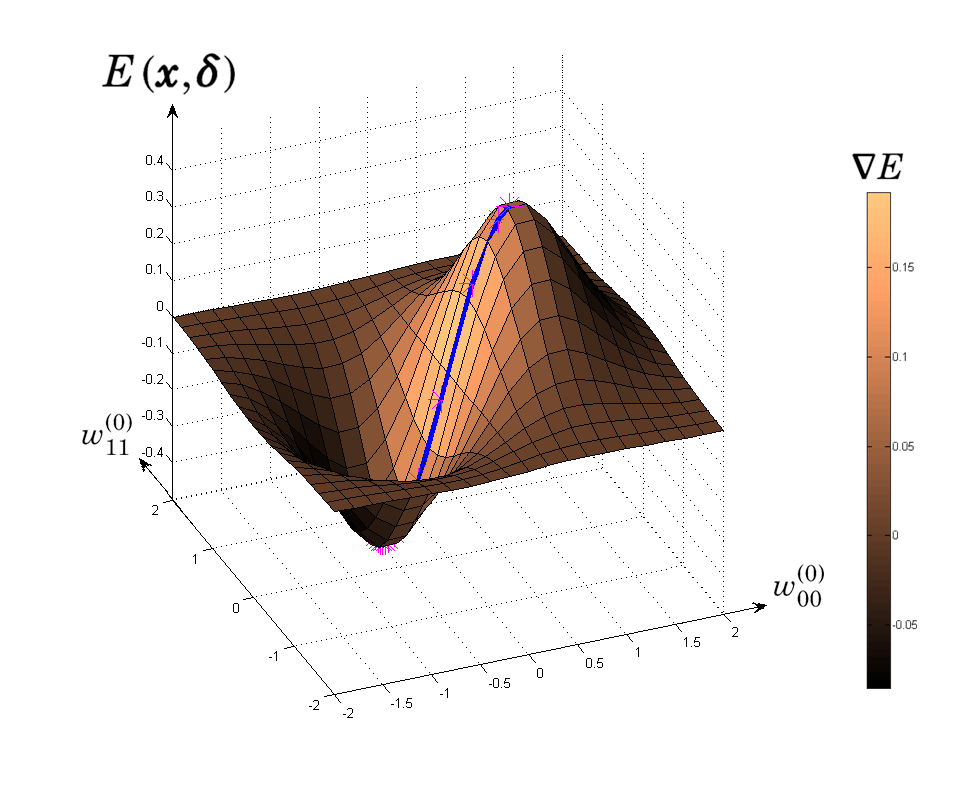
\includegraphics[width=4in]{gradient_descent}
 \caption{Gradient descent on \(E\left(\pmb{x}, \pmb{\delta}\right)\) with descent path shown in blue.}
\end{figure}
Conveniently the gradient of a function describes a vector whose direction is the greatest increase of a function. Thus to optimize our weights so that the lowest error is achieved, we update the weights as follows: \(\pmb{w}(t+1) = \pmb{w}(t)-\alpha \pmb{\nabla}E\) where alpha is some learning rate, a process which is depicted in Figure 3 \cite{rumelhart1988learning}.


The calculation of each \(\frac{\partial E}{\partial w_{ij}^{(L)}}\) is non-trivial given that each weight influences the error function in multiple ways.  To find the contribution of a single weight, recall that every single neuron is connected to all neurons in the anterior and posterior layers. So, a single weight will influence not only its posterior neuron’s sigmoidal output but also that of every neuron for any path from the posterior neuron to the set of output neurons. Thus, the multiplicity of contribution via different neural routes follows directly from the multidimensional chain-rule. Recall the differential operator \(D_g f=\frac{\partial f}{\partial x}\),
\begin{equation}
	\begin{aligned}
    \frac{\partial E}{\partial w_{ij}^{(l)}} &= D_{\sigma_0^{(L)}}\cdot D_{\mathrm{net}} \sigma_0^{(L)} \cdot D_{\sigma_0^{(L-1)}}\mathrm{net}\cdot \  \cdots \  \cdot  D_{\mathrm{net}} \sigma_j^{(l+1)} \cdot D_{w_{ij}^{(l)}}\mathrm{net} \\
    &+\  D_{\sigma_1^{(L)}}\cdot D_{\mathrm{net}} \sigma_1^{(L)} \cdot D_{\sigma_0^{(L-1)}}\mathrm{net}\cdot\  \cdots \  \cdot  D_{\mathrm{net}} \sigma_j^{(l+1)} \cdot D_{w_{ij}^{(l)}}\mathrm{net} \\
    &\ \vdots\\
    &+\  D_{\sigma_n^{(L)}}\cdot D_{\mathrm{net}} \sigma_n^{(L)} \cdot D_{\sigma_0^{(L-1)}}\mathrm{net}\cdot \  \cdots \  \cdot  D_{\mathrm{net}} \sigma_j^{(l+1)} \cdot D_{w_{ij}^{(l)}}\mathrm{net} \\
        &+\  D_{\sigma_0^{(L)}}\cdot D_{\mathrm{net}} \sigma_0^{(L)} \cdot D_{\sigma_1^{(L-1)}}\mathrm{net}\cdot \  \cdots \  \cdot  D_{\mathrm{net}} \sigma_j^{(l+1)} \cdot D_{w_{ij}^{(l)}}\mathrm{net} \\
            &\ \vdots\\
        &+\  D_{\sigma_n^{(L)}}\cdot D_{\mathrm{net}} \sigma_n^{(L)} \cdot D_{\sigma_1^{(L-1)}}\mathrm{net}\cdot \ \cdots \  \cdot  D_{\mathrm{net}} \sigma_j^{(l+1)} \cdot D_{w_{ij}^{(l)}}\mathrm{net} \\
                &\ \vdots \\
                        &+\  D_{\sigma_n^{(L)}}\cdot D_{\mathrm{net}} \sigma_n^{(L)} \cdot D_{\sigma_m^{(L-1)}}\mathrm{net}\cdot \ \cdots \ \cdot  D_{\mathrm{net}} \sigma_j^{(l+1)} \cdot D_{w_{ij}^{(l)}}\mathrm{net} \\
                        &= \sum_{a_1}^{Z^{(L)}}\ \sum_{a_2}^{Z^{(L-1)}} \cdots \sum_{a_m}^{Z^{(l+2)}} \frac{\partial E}{\partial \sigma_{a_1}^{(L)}}\frac{\partial \sigma_{a_1}^{(L)}}{\partial \mathrm{net}} \frac{\partial \mathrm{net}}{\partial \sigma_{a_2}^{(L-1)}} \ \cdots\ \frac{\partial \sigma_{a_m}^{(l+2)}}{\partial \mathrm{net}}\frac{\partial \mathrm{net}}{\partial \sigma_{j}^{(l+1)}}  \frac{\partial \sigma_{j}^{(l+1)}}{\partial \mathrm{net}} \frac{\partial \mathrm{net}}{\partial w_{ij}^{(l)}}
	\end{aligned}
\end{equation} At first sight this algorithm looks quite complicated, but a computational implementation would be able to cache certain sums and essentially reduce the complexity thereof. With the error backpropagation algorithm complete, the notion of an artificial neural network, its training, and processing is complete. Now it is possible to conjecture on variants thereof and present the primary scope of this essay.
\subsection{The Research Question}
This construction is of serious mathematical interest as feed-forward neural networks have been shown to be universal approximators; that is, they can approximate any \(f:A\to B\), where \(A,B \in \mathbb{R}^m\) are vector spaces. However it is not certain what information the approximation provides: the gradient descent algorithm does not reveal any connections between the values of the inputs.  A standing question in the field asks what can be said about the weights satisfying an approximation of $f$ besides that they exist. Therefore it is of considerable interest to explore the general form of the weights as training may not be necessary and computational complexity can be lowered.

It is the subject of this research essay to explore the neural networks through a mathematical exploration. To do this, a technique from economic mathematics is employed. It is typical that to analyze a discrete economic model, time is considered continuous and summations become integrals. To investigate neural networks then, this technique will be applied. Thus the question arises: \textbf{what can be said about artificial neural networks as the number of nodes approaches infinity and how can a real valued, continuous analogue for neural networks contribute to or aid in understanding the black box model of artificial neural networks?  }


In this paper we will generalize the notion of the universal approximation for arbitrary vector space mappings to arbitrary approximation of any \(f:L^1 (\mathbb{R}^n)\to C^\infty(\mathbb{R}^n)\) by examining the structure of feed-forward ANNs as the number of nodes for each layer becomes uncountably bounded in \(\mathbb{R}^n\). Such a generalization requires that a continuum of neural components be made, and that a continuous weight tensor or hypersurface must exist in order to maintain the topological connectedness as prescribed by the discrete model.